%=============================================================================
%  CSE 465 Project Report, North South University
%  IEEE conference format, matching the faculty sample (conference_101719).
%
%  SKELETON. Structure, tables, figures, equations and references are complete
%  and compile as they stand. Every \writehere{} is a paragraph for you to write.
%
%  Compile in Overleaf with pdfLaTeX. Run TWICE so references resolve.
%  Needs: figures/fig3_main_result.png
%         figures/fig4_truncation.png
%         figures/fig5_lengths.png
%=============================================================================
\documentclass[conference]{IEEEtran}
\IEEEoverridecommandlockouts
\usepackage{cite}
\usepackage{amsmath,amssymb,amsfonts}
\usepackage{graphicx}
\usepackage{textcomp}
\usepackage{xcolor}
\usepackage{booktabs}
\usepackage{array}
\usepackage{url}
\usepackage{tikz}
\usetikzlibrary{arrows.meta,positioning,calc}

\newcolumntype{L}[1]{>{\raggedright\arraybackslash}p{#1}}

%-----------------------------------------------------------------------------
% WRITING SLOT. Delete the whole \writehere{}{} and put your paragraph there.
% \drafttrue shows the notes. \draftfalse hides them, so set that before you
% submit and recompile to see the real page count.
%-----------------------------------------------------------------------------
\newif\ifdraft
\drafttrue

\newcommand{\writehere}[2]{%
  \ifdraft
    {\color{orange!75!black}\small\textbf{[WRITE: #1]}\itshape\ #2\par}
    \medskip
  \fi}

\begin{document}

\title{Reasoning Termination, Not Reasoning Capability,\\
Bounds Small Language Model Performance on\\
Competition Mathematics\\
{\footnotesize A budget forcing study of VibeThinker-3B on AIME 2025}
}

\author{\IEEEauthorblockN{Abu Ahmad}
\IEEEauthorblockA{\textit{Department of Electrical and Computer Engineering} \\
\textit{North South University}\\
Dhaka, Bangladesh \\
ID 2121725042}
}

\maketitle

%=============================================================================
\begin{abstract}
\writehere{Abstract, roughly 150 to 250 words}{
The IEEE template says do not use symbols, special characters, footnotes or
mathematics in the abstract, so write it in plain prose. Cover five things in
order. One, the topic: compact reasoning models now match much larger ones on
mathematics benchmarks. Two, the gap: those scores come from runs with no token
limit and nobody reports what a realistic limit costs. Three, the method: a three
billion parameter model evaluated on thirty competition problems, four samples
each, across budgets from one thousand to thirty two thousand tokens, weights
never modified, logging why every generation stopped. Four, the results: samples
that finished were almost always correct, samples cut off scored zero for want of
a written answer, and forcing the model to commit recovered seven to thirteen
points without ever destroying a correct answer. Five, the significance: any
benchmark that caps generation is measuring stopping behaviour and reporting it as
reasoning ability.}
\end{abstract}

\begin{IEEEkeywords}
large language models, mathematical reasoning, test time scaling, budget forcing,
inference efficiency, benchmark evaluation
\end{IEEEkeywords}

%=============================================================================
\section{Introduction}

\writehere{Opening, 3 paragraphs}{
One. What reasoning models are and why they improved. Reinforcement learning over
checkable rewards, cite \cite{deepseekr1} and \cite{deepseekmath}. They produce
very long chains of thought before answering.
\\
Two. VibeThinker-3B \cite{vibethinker}: three billion parameters, built on
Qwen2.5-Coder-3B \cite{qwen25coder}, reporting 91.4 on AIME 2025. Say why a model
this small mattering is interesting, that it runs on one consumer card, which puts
this kind of reasoning within reach of a student rather than only a lab with a
cluster. Your own voice belongs here.
\\
Three. The catch. Those scores come from runs with effectively no length limit;
the model card recommends a maximum of 40,960 tokens. Generating forty thousand
tokens per problem is slow on the hardware a student actually has, so the
accessibility argument contains an assumption nobody has checked.}

\writehere{The question, 1 paragraph}{
When the budget is cut and accuracy falls, what was lost? Either the model needed
those tokens to reach the answer, which is a capability failure, or it reached the
answer early and kept verifying until the budget ran out, which is a termination
failure. Say these are distinguishable by measurement and that telling them apart
is the point of this work. Then state the three constraints: no weight
modification, everything inside a free tier allowance of thirty GPU hours a week,
and every reported number measured on that hardware rather than quoted.}

The contributions of this work are as follows.

\begin{itemize}

\item \writehere{Contribution 1, the diagnosis}{
Correct count equals finished count per problem. 95 of 120 samples finished and
essentially all were correct; of the 25 truncated, 23 scored zero for want of a
parseable answer. The whole 91.4 to 80.8 shortfall is a truncation artifact.}

\item \writehere{Contribution 2, the intervention}{
Budget forcing \cite{s1} measured on a compact model at four budgets, significant
at every budget by McNemar's test, and strictly non destructive: zero correct
answers destroyed across 139 interventions.}

\item \writehere{Contribution 3, a negative result}{
Three forcing phrasings are statistically indistinguishable, and the two stage
variant costs 2.1 times more compute for no gain. What matters is that the model
is made to commit, not how it is asked.}

\item \writehere{Contribution 4, upper bounds}{
A single forced sample beats the best of four unforced samples at the smaller
budgets, so forcing exceeds the ceiling of any method that only selects among
existing answers. On the recoverable population it captures about 80 percent.}

\item \writehere{Contribution 5, the method that made it affordable}{
Prefix consistency. Generation is autoregressive, so the first N tokens of a long
run are what a budget N run would have produced. Generate once at the top budget,
score every smaller budget on CPU at no GPU cost. Validated, not assumed.}

\end{itemize}

\writehere{Roadmap, 2 or 3 sentences}{
One sentence per section, from Section II to Section VII.}

%=============================================================================
\section{Background Work and Literature Review}

\subsection{Reinforcement learning for verifiable reasoning}

\writehere{2 paragraphs}{
First, DeepSeek-R1 \cite{deepseekr1} and the GRPO objective from DeepSeekMath
\cite{deepseekmath}: rule based reinforcement learning over checkable rewards
produces long horizon reasoning with no step level supervision.
\\
Second, VibeThinker-3B \cite{vibethinker} in the small model regime. Two facts
matter here. Their evaluation imposes no output length cap, and their reported
weakness is knowledge heavy tasks rather than reasoning procedure. Then say what
is missing: neither the paper nor the model card reports how accuracy degrades
under a constrained budget, which is the regime anyone on modest hardware
occupies.}

\subsection{Inference time scaling}

\writehere{2 paragraphs}{
Self consistency \cite{selfconsistency} samples several chains and takes the
majority. Self refinement \cite{selfrefine} has the model critique and revise its
own output. VibeThinker's paper describes Claim Level Reliability Assessment.
\\
Then the structural point that carries your argument. All three select or refine
among candidate answers that already exist, so their achievable accuracy is
bounded by pass@k. Where samples agree, or produce no answer at all, they have
nothing to act on. Say Section V shows this bound is binding here.}

\subsection{Budget forcing}

\writehere{1 paragraph}{
Muennighoff et al. \cite{s1} introduced budget forcing: on reaching a token budget,
append a phrase that ends the reasoning segment and demands an answer. Note what
they did not do, since that is where this work sits. They use it mainly to extend
reasoning, combined with supervised fine tuning, so its use as a standalone
recovery mechanism on a frozen model is not characterised, and nobody measures
whether it can damage an output.}

\subsection{The gap}

\writehere{1 paragraph, then the four items}{
Introduce the list in one sentence.}

\begin{enumerate}
\item \writehere{Gap 1}{Published accuracies come from uncapped runs and the
degradation curve under realistic budgets is not characterised, though deployment
cost is the main argument for compact models.}
\item \writehere{Gap 2}{Failure analyses report aggregate accuracy without
separating a wrong answer from an absent one, so two failure modes with different
remedies score identically at zero.}
\item \writehere{Gap 3}{Test time scaling methods are evaluated where samples
disagree, so their behaviour where samples agree or produce nothing is untested.}
\item \writehere{Gap 4}{Budget forcing has been evaluated as an extension
mechanism alongside fine tuning, not as a standalone recovery mechanism on a
frozen model, and no measurement exists of whether it can destroy a correct
output.}
\end{enumerate}

%=============================================================================
\section{Proposed Methodology}

\subsection{Problem formulation}

Let $\pi$ be the frozen policy and $q$ a problem statement. Under an unconstrained
budget the model emits $y = (y_1,\dots,y_T)$ ending in an end of sequence token,
and an answer $a(y)$ is parsed from the final boxed expression. Under a budget $B$
the generation is cut at $\min(T,B)$ tokens. Define the termination indicator

\begin{equation}
\tau_B(y) =
\begin{cases}
1, & T \le B \\
0, & T > B
\end{cases}
\label{eq:tau}
\end{equation}

and the correctness indicator
$c_B(y) = \mathbb{1}[\,a(y_{1:\min(T,B)}) = a^{\star}\,]$, where $a^{\star}$ is
the ground truth.

\writehere{1 paragraph}{
Under the capability hypothesis, truncated traces are wrong because the reasoning
is incomplete, so correctness should fall smoothly across both groups. Under the
termination hypothesis, correctness should be near total among terminated samples
and near zero among truncated ones, as in (\ref{eq:hyp}). Say this is what makes
the two distinguishable by measurement.}

\begin{equation}
\Pr[c_B = 1 \mid \tau_B = 1] \approx 1, \quad
\Pr[c_B = 1 \mid \tau_B = 0] \approx 0
\label{eq:hyp}
\end{equation}

\subsection{Budget forcing}

\writehere{1 paragraph}{
Describe the procedure before the equation. Forcing acts only on truncated
samples: take the truncated prefix, append a fixed phrase that closes the
reasoning block and asks for the answer, decode greedily for a short continuation.
Samples that terminated on their own are left untouched, and say explicitly that
this is why the method cannot damage them. The cost is about five generated tokens
per intervened sample.}

\begin{equation}
\hat{a} = a\!\left(\pi\!\left(q \oplus y_{1:B} \oplus \phi\right)\right)
\label{eq:forcing}
\end{equation}

\writehere{2 sentences on the three variants}{
Name them: a bare demand $V_1$, a soft deadline $V_3$, and a two stage variant
$V_2$ where the model first summarises what it established and only then is asked
for the answer. Say why three rather than one.}

\subsection{Prefix consistency}

\writehere{1 paragraph}{
Explain (\ref{eq:prefix}) in plain words: the model generates left to right and
has no knowledge of its own budget, so the distribution of the first N tokens does
not depend on where generation was stopped. The consequence is that saving traces
at the top budget lets every smaller budget be scored on CPU at no GPU cost.
Validated in Section IV rather than assumed.}

\begin{equation}
y_{1:N} \Big|_{\text{budget } N}
\;\overset{d}{=}\;
\left(y \Big|_{\text{budget } B}\right)_{1:N},
\quad N \le B
\label{eq:prefix}
\end{equation}

\subsection{Statistical procedure}

\writehere{1 paragraph}{
The design is paired because the same samples are scored twice, before and after
the intervention, so an unpaired test would be the wrong tool. McNemar with
continuity correction \cite{mcnemar}, shown in (\ref{eq:mcnemar}), where $b$ is
samples that changed from incorrect to correct and $c$ the reverse. Say $c$ is of
independent interest because it measures whether the intervention can destroy a
correct answer. Wilson intervals \cite{wilson} for the ceiling proportions,
because the denominators are small.}

\begin{equation}
\chi^{2} = \frac{\left(|b - c| - 1\right)^{2}}{b + c}
\label{eq:mcnemar}
\end{equation}

\subsection{System design}

\writehere{1 short paragraph introducing Fig. \ref{fig:pipeline}}{
Two or three sentences: generate once, truncate on CPU to reach each budget,
score, force only the truncated samples, analyse.}

\begin{figure*}[t]
\centering
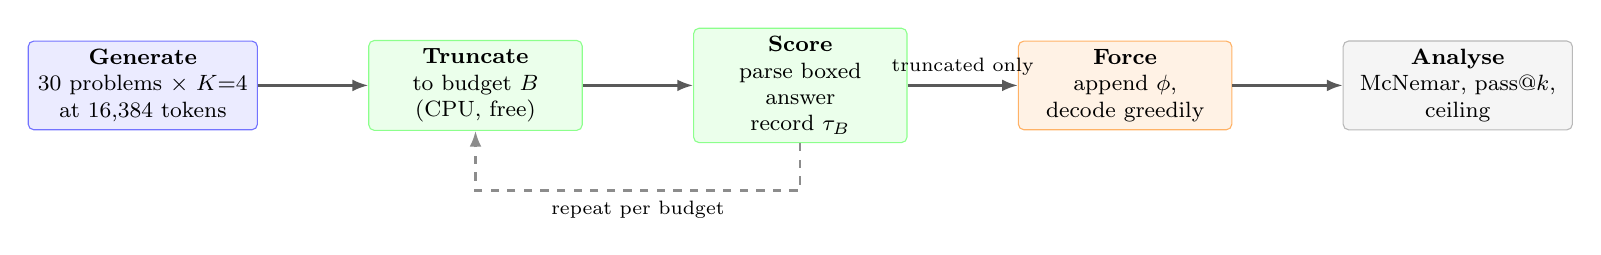
\begin{tikzpicture}[
  node distance=7mm,
  box/.style={draw,rounded corners=2pt,align=center,minimum height=10mm,
              inner sep=3pt,font=\footnotesize},
  gen/.style={box,fill=blue!8,draw=blue!55,text width=27mm},
  cpu/.style={box,fill=green!8,draw=green!45,text width=25mm},
  gpu/.style={box,fill=orange!10,draw=orange!60,text width=25mm},
  ana/.style={box,fill=gray!8,draw=gray!55,text width=27mm},
  ar/.style={-{Latex[length=2mm]},thick,draw=black!65}
]
\node[gen] (gen) {\textbf{Generate}\\30 problems $\times$ $K{=}4$\\at 16{,}384 tokens};
\node[cpu, right=14mm of gen] (trunc) {\textbf{Truncate}\\to budget $B$\\(CPU, free)};
\node[cpu, right=14mm of trunc] (score) {\textbf{Score}\\parse boxed answer\\record $\tau_B$};
\node[gpu, right=14mm of score] (force) {\textbf{Force}\\append $\phi$,\\decode greedily};
\node[ana, right=14mm of force] (stats) {\textbf{Analyse}\\McNemar, pass@$k$,\\ceiling};

\draw[ar] (gen) -- (trunc);
\draw[ar] (trunc) -- (score);
\draw[ar] (score) -- node[above,font=\scriptsize]{truncated only} (force);
\draw[ar] (force) -- (stats);
\draw[ar,dashed,draw=black!45] (score.south) -- ++(0,-6mm) -| (trunc.south)
      node[below,font=\scriptsize,pos=0.25]{repeat per budget};
\end{tikzpicture}
\caption{Experimental pipeline. Generation runs once at the largest budget.
Smaller budgets come from truncating the stored traces on a CPU, which costs
nothing. Only the forcing step returns to the GPU, and it acts on truncated
samples alone.}
\label{fig:pipeline}
\end{figure*}

%=============================================================================
\section{Experiments}

\subsection{Model, dataset and hardware}

\writehere{2 paragraphs}{
First: the model and the dataset. VibeThinker-3B, weights never modified, and the
30 problem AIME 2025 set. Explain the substitution honestly because a reader will
ask: AIME 2026 has no public dataset, so AIME 2025 was used, and this is an
advantage since the paper reports 91.4 for AIME 2025 and it allows the harness to
be validated. Integer answers between 0 and 999 mean exact matching with no judge
model.
\\
Second: the engine. HuggingFace transformers gave 15.2 tokens per second, which
projected to over a hundred GPU hours and was not feasible. vLLM \cite{vllm}
raised it to 246.4 at $K{=}32$, a 16.2 times improvement, through continuous
batching and prefix sharing. Point at Table \ref{tab:tools}.}

\begin{table*}[t]
\caption{Software and Hardware Components}
\label{tab:tools}
\centering
\footnotesize
\begin{tabular}{@{}L{2.4cm}L{3.4cm}L{3.4cm}L{6.4cm}@{}}
\toprule
\textbf{Tool} & \textbf{Function} & \textbf{Alternatives} & \textbf{Reason selected} \\
\midrule
vLLM & Inference engine & HF \texttt{transformers}, TensorRT-LLM &
$16.2\times$ faster through continuous batching and prefix sharing; the workload
is many samples from one prompt, its best case \\
\addlinespace
Tesla T4, 16\,GB & Accelerator & A100, TPU v4 & The only hardware on the free
tier; forces \texttt{float16} and rules out FlashAttention-2 \\
\addlinespace
VibeThinker-3B & Subject model & Qwen3-4B, Phi-4-mini & Frontier accuracy at 3B; a
published AIME 2025 score allows harness validation \\
\addlinespace
\texttt{math-ai/aime25} & Benchmark & AIME 2024, HMMT & Integer answers allow
exact matching against a published reference number \\
\addlinespace
Kaggle Notebooks & Compute platform & Colab, Lambda Labs & 30 GPU hours per week
at no cost; batch execution survives disconnection \\
\bottomrule
\end{tabular}
\end{table*}

\writehere{1 paragraph on the T4 constraints}{
Three consequences of the card being Turing, compute capability 7.5.
FlashAttention-2 needs 8.0 or above so vLLM falls back to a Triton backend.
bfloat16 is unsupported so float16 is mandatory. And the key value cache holds
192,272 tokens at 90 percent utilisation, so concurrency is that divided by the
context window as in (\ref{eq:conc}), which is why a 32k context sustained 60 to
71 tokens per second while an 8k context sustained 246.}

\begin{equation}
\text{concurrency} = \frac{192{,}272}{\texttt{max\_model\_len}}
\label{eq:conc}
\end{equation}

\subsection{Protocol}

\writehere{2 paragraphs}{
One: the controls. Decoding parameters frozen across every arm, temperature 1.0,
top-p 0.95, seed 0, $K$ equals 4 giving 120 samples per condition. Prompt from the
model's own chat template. Answer extraction finds the final boxed expression with
a brace depth parser. One shared implementation across all arms so a change cannot
apply to only one condition. Budgets of 4,096, 8,192, 16,384 and 32,768 tokens.
\\
Two: termination logging, and why it is the important part. Separating a wrong
answer from an absent one is what makes (\ref{eq:hyp}) testable. Aggregate accuracy
alone cannot support the central claim, which is why the harness records a stop
reason for every sample.}

\subsection{Compute expenditure}

\begin{table}[t]
\caption{Measured Compute Expenditure}
\label{tab:compute}
\centering
\footnotesize
\begin{tabular}{@{}L{3.1cm}rL{3.4cm}@{}}
\toprule
\textbf{Stage} & \textbf{GPU h} & \textbf{Purpose} \\
\midrule
Setup and probes & 1.50 & Environment audit, throughput \\
Baseline, 32K & 8.87 & 30 problems, $K{=}4$ \\
Forcing, 4K and 8K & 2.06 & First forcing measurement \\
Forcing variants, 16K & 8.89 & Traces and six forcing passes \\
Trace analysis & 0.00 & CPU only; curve and figures \\
Paired analysis & 1.28 & McNemar at 8K and 16K \\
Upper bounds & 0.00 & CPU only; pass@$k$, ceiling \\
\midrule
\textbf{Total} & \textbf{22.60} & \\
\bottomrule
\end{tabular}
\end{table}

\subsection{Harness validation}

\writehere{2 paragraphs}{
First check: the baseline reproduction gave 80.8 against the published 91.4. The
direction matters, so say it: the figure is lower, which argues against
contamination inflating anything.
\\
Second check: the identity in (\ref{eq:prefix}) tested directly. An 8,192 token
condition measured two ways, a genuine 8k run and truncated 16k traces, gave 54.2
and 55.8 percent. Two samples out of 120, within noise at temperature 1.0. Every
later budget result depends on this holding.}

%=============================================================================
\section{Results}

\subsection{Termination against correctness}

\begin{table}[t]
\caption{Correct Against Naturally Terminated Samples, 32K Budget}
\label{tab:decomp}
\centering
\footnotesize
\begin{tabular}{@{}crrl@{}}
\toprule
\textbf{Problem} & \textbf{Correct} & \textbf{Terminated} & \textbf{Note} \\
\midrule
8  & 2/4 & 2/4 & \\
13 & 0/4 & 0/4 & all truncated \\
14 & 0/4 & 0/4 & all truncated \\
19 & 2/4 & 2/4 & \\
26 & 3/4 & 3/4 & \\
27 & 1/4 & 1/4 & \\
29 & 0/4 & 0/4 & all truncated \\
\midrule
21 problems & 4/4 & 4/4 & solved by all \\
\bottomrule
\end{tabular}
\end{table}

\writehere{1 paragraph, arithmetic only, interpretation goes in Section VI}{
All 21 fully solved problems also terminated on all four samples, contributing 84
samples. Aggregating, 97 correct and 95 terminated, so among the 95 that
terminated essentially every one was correct. Of the 25 truncated, 23 scored zero.
Keep it factual here.}

\subsection{Accuracy against budget}

\begin{figure*}[t]
\centering
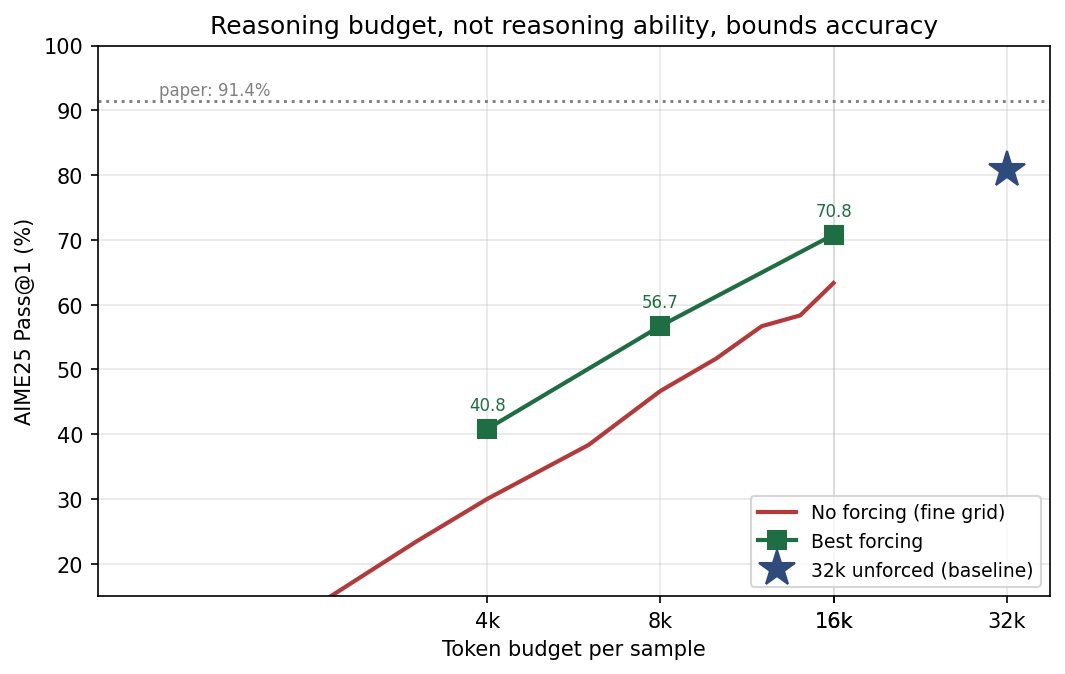
\includegraphics[width=0.82\textwidth]{figures/fig3_main_result.png}
\caption{Accuracy against generation budget, with and without budget forcing. The
dotted line marks the accuracy reported in \cite{vibethinker} under an
unconstrained budget.}
\label{fig:main}
\end{figure*}

\begin{table}[t]
\caption{Accuracy and Truncation Against Budget, No Forcing}
\label{tab:curve}
\centering
\footnotesize
\begin{tabular}{@{}rrr@{\hspace{1.4em}}rrr@{}}
\toprule
\textbf{Budget} & \textbf{Pass@1} & \textbf{Trunc.} &
\textbf{Budget} & \textbf{Pass@1} & \textbf{Trunc.} \\
\midrule
1K & 3.3\%  & 100.0\% & 8K  & 46.7\% & 67.5\% \\
2K & 13.3\% & 98.3\%  & 10K & 51.7\% & 63.3\% \\
3K & 23.3\% & 92.5\%  & 12K & 56.7\% & 59.2\% \\
4K & 30.0\% & 87.5\%  & 14K & 58.3\% & 53.3\% \\
6K & 38.3\% & 77.5\%  & 16K & 63.3\% & 48.3\% \\
\bottomrule
\end{tabular}
\end{table}

\begin{figure}[t]
\centering
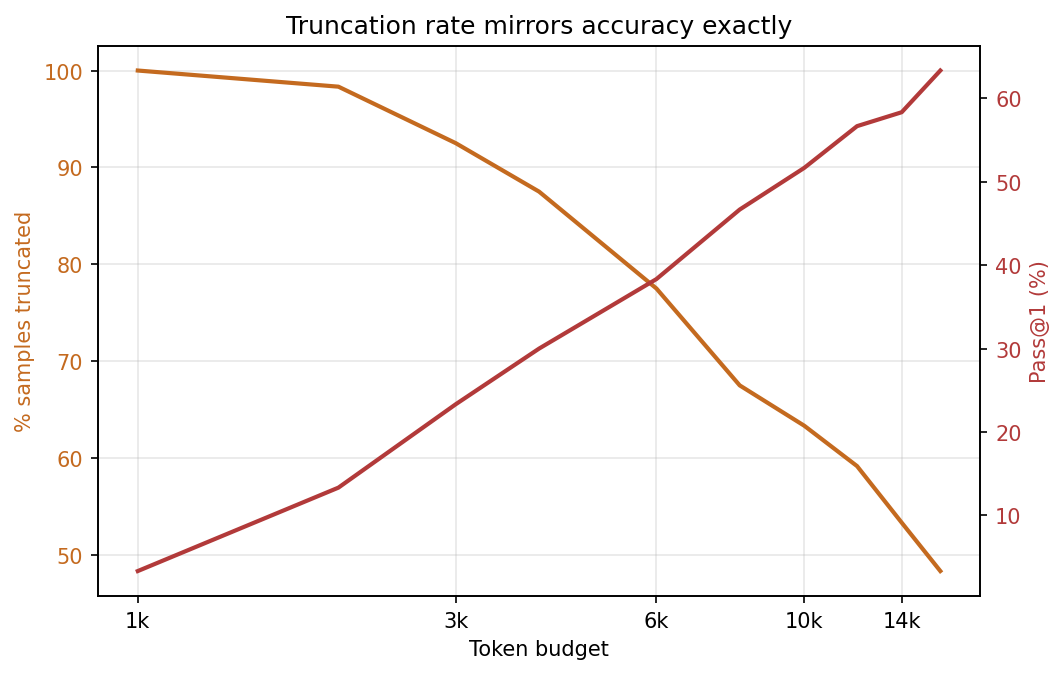
\includegraphics[width=\columnwidth]{figures/fig4_truncation.png}
\caption{Truncation rate and accuracy move inversely with budget. Left axis, the
percentage of samples cut off. Right axis, Pass@1 over the same samples.}
\label{fig:trunc}
\end{figure}

\writehere{1 paragraph}{
State the curve, then note one thing a reader will otherwise miss: accuracy
exceeds the natural termination rate by 12 to 18 points at every budget, because
the model sometimes writes an intermediate boxed expression mid derivation which
the parser recovers even though the trace never terminated. The unforced baseline
therefore already captures some truncated but answered samples.}

\begin{figure}[t]
\centering
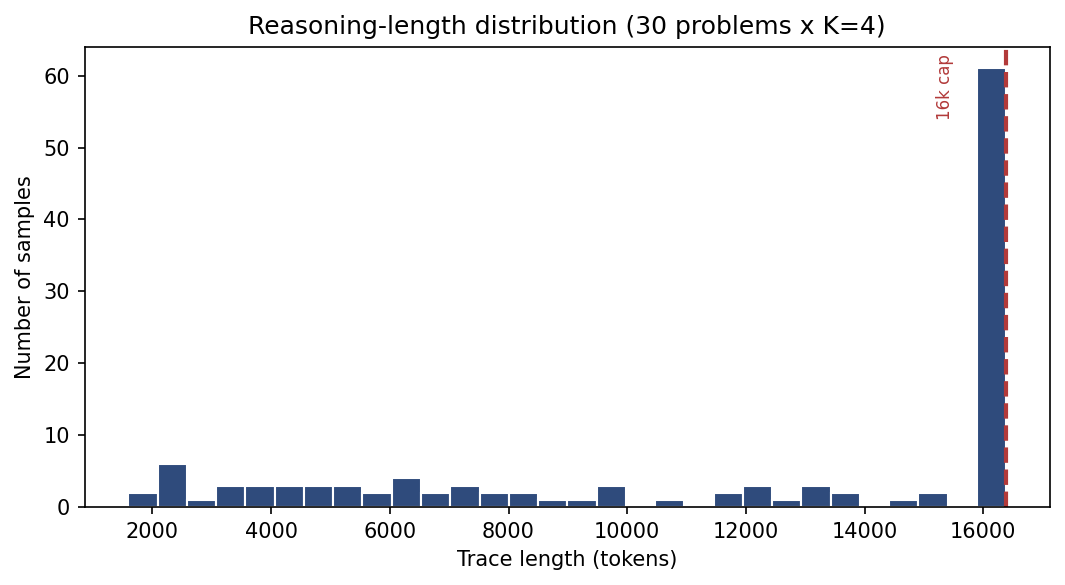
\includegraphics[width=\columnwidth]{figures/fig5_lengths.png}
\caption{Distribution of reasoning trace lengths over 30 problems and four samples
each. The distribution is right censored at 16{,}384 tokens; the mass at the cap
is an artifact of the imposed limit, not the model stopping on its own.}
\label{fig:lengths}
\end{figure}

\subsection{Effect of budget forcing}

\begin{table}[t]
\caption{Effect of Budget Forcing on AIME 2025 Pass@1}
\label{tab:main}
\centering
\footnotesize
\begin{tabular}{@{}lrrrc@{}}
\toprule
\textbf{Budget} & \textbf{No forcing} & \textbf{Forced} & \textbf{Gain} &
\textbf{McNemar $p$} \\
\midrule
4K  & 27.5 / 30.0\% & 40.8\% & $+13.3$ & not run \\
8K  & 46.7\%        & 55.8\% & $+9.1$  & $\mathbf{0.0026}$ \\
16K & 63.3\%        & 70.8\% & $+7.5$  & $\mathbf{0.0077}$ \\
32K & 80.8\%        & n/m    &         & \\
\bottomrule
\end{tabular}
\end{table}

\writehere{1 paragraph}{
The gain is significant at every budget where the paired test could be applied.
Explain the two baselines in the 4K row honestly: that budget was measured twice,
once by a dedicated run at 27.5 percent and once by truncating traces at 30.0
percent. Three samples apart, within noise, but different experiments, so they
should not be plotted as one series.}

\subsection{Test for harm}

\begin{table}[t]
\caption{Paired Contingency, Truncated Samples Only}
\label{tab:paired}
\centering
\footnotesize
\begin{tabular}{@{}lrrrrrr@{}}
\toprule
\textbf{Budget} & \textbf{Trunc.} & \textbf{$b$} & \textbf{$c$} &
\textbf{r$\rightarrow$r} & \textbf{$\chi^2$} & \textbf{$p$} \\
\midrule
8K  & 81 & 11 & \textbf{0} & 17 & 9.09 & 0.0026 \\
16K & 58 & 9  & \textbf{0} & 14 & 7.11 & 0.0077 \\
\bottomrule
\end{tabular}
\end{table}

\writehere{1 paragraph, factual}{
Across 139 interventions $c$ equals zero. Note that 31 truncated traces already
contained a correct boxed expression and forcing re derived the identical value
for every one. Save the explanation for Section VI.}

\subsection{Sensitivity to the forcing phrase}

\begin{table}[t]
\caption{Comparison of Forcing Phrasings}
\label{tab:variants}
\centering
\footnotesize
\begin{tabular}{@{}lrrr@{\hspace{1.2em}}rr@{}}
\toprule
& \multicolumn{3}{c}{\textbf{Pass@1}} & \multicolumn{2}{c}{\textbf{Cost, min}} \\
\cmidrule(lr){2-4}\cmidrule(l){5-6}
\textbf{Budget} & $V_1$ & $V_3$ & $V_2$ & $V_1$ & $V_2$ \\
\midrule
8K  & 55.8\% & 55.8\% & 56.7\% & 21.2 & 47.8 \\
16K & 70.8\% & 70.8\% & 70.8\% & 54.9 & 117.3 \\
\bottomrule
\end{tabular}
\end{table}

\writehere{1 paragraph, factual}{
Identical at 16K. The 0.9 point lead at 8K is one sample out of 120. $V_2$ costs
2.1 times more compute at both budgets.}

\subsection{Upper bounds}

\begin{table}[t]
\caption{Budget Forcing Against the Selection Oracle}
\label{tab:oracle}
\centering
\footnotesize
\begin{tabular}{@{}lrr@{}}
\toprule
\textbf{Budget} & \textbf{Unforced pass@4} & \textbf{Forced pass@1} \\
\midrule
4K  & 40.0\% & \textbf{40.8\%} \\
8K  & 53.3\% & \textbf{55.8\%} \\
16K & \textbf{73.3\%} & 70.8\% \\
\bottomrule
\end{tabular}
\end{table}

\begin{table*}[t]
\caption{Extraction Ceiling on the Recoverable Population}
\label{tab:ceiling}
\centering
\footnotesize
\begin{tabular}{@{}lrrrrrrrr@{}}
\toprule
\textbf{Budget} & \textbf{Truncated} & \textbf{Already correct} &
\textbf{Rescuable} & \textbf{Has answer} & \textbf{False pos.} &
\textbf{Ceiling} & \textbf{Rescued} & \textbf{Captured} \\
\midrule
8K  & 81 & 17 & 64 & 16 & 2 & 14 & 11 & 78.6\% \\
16K & 58 & 14 & 44 & 11 & 0 & 11 &  9 & 81.8\% \\
\bottomrule
\end{tabular}
\end{table*}

\writehere{2 paragraphs, factual}{
One: at 4K and 8K a single forced sample beats the best of four unforced ones; at
16K the ordering reverses. State the caveat, that this compares forced pass@1
against unforced pass@4 and forced pass@4 was not computed.
\\
Two: forcing captures 78.6 percent at 8K and 81.8 at 16K of the recoverable
population, with Wilson intervals of roughly 52 to 92 and 52 to 95 on populations
of 14 and 11. The false positive control ran 0 to 4.9 percent against a signal of
32 to 41 percent. Only 16 of 64 rescuable traces at 8K and 11 of 44 at 16K mention
the correct answer anywhere in their final fifth.}

%=============================================================================
\section{Analysis}

\subsection{Termination, not capability}

\writehere{2 paragraphs}{
First: interpret Table \ref{tab:decomp}. The pattern is what (\ref{eq:hyp})
predicts under the termination hypothesis and is inconsistent with the capability
hypothesis, which predicts smooth degradation across both groups. So the 91.4 to
80.8 shortfall is a truncation artifact rather than a reasoning deficit.
\\
Second: the worked example, which is the most convincing thing in the paper.
Problem 1, answer 588. The model derives $AB = 28$ and $AC = 91$, sets up
coordinates, concludes the heptagon area equals the triangle area, and the value
588 appears in its working. Then it keeps verifying and never writes a boxed
answer before the budget expires. The reasoning succeeded. Only the act of stating
the result failed.}

\subsection{Why forcing cannot do harm}

\writehere{2 paragraphs}{
First: explain the zero using the right to right column. Thirty one truncated
traces already contained a correct boxed expression, and forcing overwrote every
one and re derived the identical value. Once the model has established a result
firmly enough to state it once, being made to state it again reproduces it,
because the working is still in its context.
\\
Second: the consequence. A hybrid policy that preserves an existing answer and
forces only when none is present scores identically, so the extra logic is
unnecessary. Say it was built and discarded, because that is what happened.}

\subsection{Why the phrasing does not matter}

\writehere{2 paragraphs}{
First: interpret Table \ref{tab:variants}. What the intervention supplies is
permission to stop, not a better prompt, so elaborating the request adds cost
without adding information. The information the model needs is already in its own
trace.
\\
Second: the cost caveat, and be careful here. Forcing's wall clock cost is
dominated by prefill, re reading the stored trace, because the forcing step itself
generates about five tokens. An implementation that kept the key value cache would
make forcing nearly free, so these timings are not an intrinsic cost of the
method.}

\subsection{What forcing can and cannot recover}

\writehere{3 paragraphs}{
One: the two worked examples together. Problem 1, answer 588, where three of four
summaries contain genuine derived quantities and forcing yields 588. Problem 13,
answer 60, where the summaries are still setting up the problem and forcing yields
confident but wrong values of 124 and 184.
\\
Two: the generalisation. Budget forcing recovers answers already latent in the
trace and cannot manufacture reasoning that has not occurred. Show that this one
statement accounts for all four findings: the gain is real because latent answers
are common, the gain is bounded because most failures are genuinely incomplete,
forcing is non destructive because a latent answer is stable under re elicitation,
and the phrasing is irrelevant because what is supplied is permission to conclude.
\\
Three: where the headroom is. Only about a quarter of rescuable traces mention the
answer at all, so roughly three quarters of failures never derived it and no
extraction procedure could recover them. The remaining opportunity is in generating
reasoning, not reading it out.}

\subsection{Implications for evaluation practice}

\writehere{1 paragraph, and say what you actually think}{
Any benchmark that caps generation on a long horizon reasoning model measures a
composite of reasoning ability and stopping behaviour and reports it as reasoning
ability alone. Under such protocols this cheap intervention is worth 7 to 13
points, which is larger than the margin separating many published systems. A
judgement of your own belongs here.}

%=============================================================================
\section{Conclusion}

\writehere{2 paragraphs}{
One: restate the question and the answer. Whether the accuracy loss under a
constrained budget reflects a failure of reasoning or of termination, and the two
separate cleanly: samples that terminated were almost always correct, truncated
samples scored zero for want of a written answer.
\\
Two: what forcing achieved. 7.5 to 13.3 points, significant at every budget by
McNemar, never converted a correct answer into an incorrect one across 139
interventions, three phrasings indistinguishable, a single forced sample beating
the best of four unforced ones at the smaller budgets, and roughly 80 percent of
recoverable answers captured. End on the compute figure: 22.6 GPU hours on freely
available hardware.}

\subsection{Limitations}

\writehere{1 paragraph covering all of these, or a short list}{
One model, one benchmark, one seed, with binomial intervals over 120 samples and
no run to run variance estimate, so the defensible claim is that the effect
exceeds plausible sampling noise rather than that it replicates. $K$ equals 4 is
small. The extraction ceiling rests on 11 to 14 samples so its interval spans
roughly 52 to 95 percent. AIME 2026 was unavailable publicly so AIME 2025 was
used, which predates the subject publication and sat inside its evaluation scope,
and no independent decontamination check was run. \texttt{max\_model\_len} differed
across arms for memory reasons and was not controlled. Forcing's cost figures are
implementation bound. Forcing at 32K and forced pass@4 were not measured. And an
earlier ceiling estimate was retracted after its denominator proved to coincide
with the already correct set. Keep that last one in.}

\subsection{Future work}

\writehere{1 paragraph, four directions}{
Cache reusing forcing, which would cut the cost to roughly the five tokens it
actually generates. Learned termination, since about three quarters of failures
never derive the answer, making the model conclude sooner addresses the cause
rather than the symptom. Generality, whether the decomposition holds for other
compact reasoning models and on code generation as well as mathematics. And
evaluation protocol, since publishing the truncation rate alongside accuracy would
cost nothing and make results across different budgets comparable.}

%=============================================================================
\section*{Code and Data Availability}

The analysis code, the measured result files and all 120 reasoning traces are held
in the project repository at
\url{https://github.com/abuahmad369/llm-budget-forcing}.
A public write up with the result files and an interactive explorer holding all
120 traces is available at
\url{https://github.com/abuahmad369/reasoning-termination}
and \url{https://abuahmad369.github.io/reasoning-termination/}.

%=============================================================================
\begin{thebibliography}{00}

\bibitem{vibethinker}
S. Xu, S. Liu, W. Wang, J. Min, Y. Dai, Z. Yin, Y. Chen, X. Zhou, and J. Zhang,
``VibeThinker-3B: Exploring the frontier of verifiable reasoning in small language
models,'' arXiv preprint arXiv:2606.16140, 2026.

\bibitem{s1}
N. Muennighoff, Z. Yang, W. Shi, X. L. Li, L. Fei-Fei, H. Hajishirzi,
L. Zettlemoyer, P. Liang, E. Cand\`{e}s, and T. Hashimoto, ``s1: Simple test time
scaling,'' arXiv preprint arXiv:2501.19393, 2025.

\bibitem{deepseekr1}
D. Guo, D. Yang, H. Zhang, J. Song, R. Zhang, R. Xu, Q. Zhu, S. Ma, P. Wang, and
X. Bi, ``DeepSeek-R1: Incentivizing reasoning capability in LLMs via reinforcement
learning,'' arXiv preprint arXiv:2501.12948, 2025.

\bibitem{deepseekmath}
Z. Shao, P. Wang, Q. Zhu, R. Xu, J. Song, X. Bi, H. Zhang, M. Zhang, Y. K. Li, and
Y. Wu, ``DeepSeekMath: Pushing the limits of mathematical reasoning in open
language models,'' arXiv preprint arXiv:2402.03300, 2024.

\bibitem{selfconsistency}
X. Wang, J. Wei, D. Schuurmans, Q. Le, E. Chi, S. Narang, A. Chowdhery, and
D. Zhou, ``Self consistency improves chain of thought reasoning in language
models,'' in \emph{Proc. Int. Conf. Learning Representations}, 2023.

\bibitem{selfrefine}
A. Madaan, N. Tandon, P. Gupta, S. Hallinan, L. Gao, S. Wiegreffe, U. Alon,
N. Dziri, S. Prabhumoye, and Y. Yang, ``Self-Refine: Iterative refinement with self
feedback,'' in \emph{Advances in Neural Information Processing Systems}, vol. 36,
2023, pp. 46534--46594.

\bibitem{qwen25coder}
B. Hui, J. Yang, Z. Cui, J. Yang, D. Liu, L. Zhang, T. Liu, J. Zhang, B. Yu, and
K. Dang, ``Qwen2.5-Coder technical report,'' arXiv preprint arXiv:2409.12186, 2024.

\bibitem{vllm}
W. Kwon, Z. Li, S. Zhuang, Y. Sheng, L. Zheng, C. H. Yu, J. Gonzalez, H. Zhang, and
I. Stoica, ``Efficient memory management for large language model serving with
PagedAttention,'' in \emph{Proc. 29th Symp. Operating Systems Principles}, 2023,
pp. 611--626.

\bibitem{mcnemar}
Q. McNemar, ``Note on the sampling error of the difference between correlated
proportions or percentages,'' \emph{Psychometrika}, vol. 12, no. 2, pp. 153--157,
1947.

\bibitem{wilson}
E. B. Wilson, ``Probable inference, the law of succession, and statistical
inference,'' \emph{J. Amer. Statist. Assoc.}, vol. 22, no. 158, pp. 209--212, 1927.

\end{thebibliography}

\end{document}
